\documentclass[a4paper,10pt]{article}

\usepackage[inner=3cm,top=3cm,outer=3cm,bottom=3cm]{geometry}
\usepackage[parfill]{parskip} % line skip between paragraphs instead of indents
\usepackage{fancyhdr}
\usepackage{fancyvrb}
\usepackage{graphicx}
\usepackage{xcolor}
\usepackage{color, colortbl}
\usepackage{setspace} % dynamic line spacing
\usepackage{float} % picture placing
\usepackage{caption}
\usepackage{verbatim} % insert files verbatim
\usepackage{pdfpages} % import raw pdf
\usepackage[toc,page]{appendix}
\usepackage[labelformat=empty]{caption} % picture captions
\ifxetex
  % babel for xetex
  \usepackage{fontspec}
  \usepackage{polyglossia}
  \setdefaultlanguage{swedish}
	% i xetex behövs inga fulhack för åäö
\else
	% åäö-hax för icke-xelatex
  \usepackage[swedish]{babel}
	\usepackage[utf8]{inputenc}
  \usepackage[T1]{fontenc}
\fi
\usepackage[style=authoryear,backend=biber]{biblatex} % harvard citing, modern backend
\usepackage{csquotes} % language aware quoting
\usepackage{hyperref} % automatic pdf bookmarks and hyperlinks, must be loaded last

\bibliography{reference} % link to bibliography bib file

% Header and footer
\pagestyle{fancy}\headheight 13pt
\fancyfoot{} % reset footer format
\fancyfoot[LE,RO]{\thepage}
\renewcommand{\headrulewidth}{0pt}
\renewcommand{\footrulewidth}{0pt}

% configuration
\def\thetitle{URD-2}
\def\groupname{The Meta Family}
\def\groupmembers{Daniel Bergström \\ Paulina Hensman \\ Marcus Hertz \\ Simon Karlsson \\ David Masko \\ Marcus Nordberg \\ André Nyström \\ William Perkola \\ Axel Riese \\ Kerry Zhang}
\def\version{Version 2.0}
\def\thedate{\today}
\renewcommand{\arraystretch}{1.2} % spacious tables

%----------------------------------------------------------------------------------------
%	TITLE PAGE
%----------------------------------------------------------------------------------------

\newcommand*{\titleGM}{\begingroup % Create the command for including the title page in the document
\hbox{ % Horizontal box
\hspace*{0.1\textwidth} % Whitespace to the left of the title page
\parbox[b]{0.75\textwidth}{ % Paragraph box which restricts text to less than the width of the page

{\noindent\Huge\bfseries \thetitle \\[0.5\baselineskip] \groupname}\\[2\baselineskip] % Title

{\large \version \\[\baselineskip] den \thedate}\\[2\baselineskip] 

\begin{doublespace}
{\Large \groupmembers} % Author name
\end{doublespace}

}}
\endgroup}


% pdf metadata
\hypersetup{pdfinfo={
Title={ADD},
Author={The Meta Family}
}}

\begin{document}

% title page
\thispagestyle{empty}
\titleGM
\clearpage

% empty/icon page
\thispagestyle{empty}

\includepdf{metafam.pdf}
\clearpage 

% abstract
\thispagestyle{empty}
\section*{Sammanfattning} %unnumbered
Denna projektplaneringsrapport behandlar implementeringen av en SDK (Software development kit) till Android för applikationstestning.
\clearpage

% table of contents
% generated automatically
% from \section commands
\thispagestyle{empty}
\tableofcontents % babel/polyglossia fixar språket
\clearpage

% document change record
\setcounter{page}{1}
\section*{Versionshistorik}
% add to table of contents, but no numbering
\addcontentsline{toc}{section}{Versionshistorik}
\subsection*{0.1}
Första utkast. Varje underrubrik utom abstract är färdigskriven men texten är ej korrekturläst.

\subsection*{0.2}
Rapporten har uppdaterats med ett abstract.

\subsection*{1.0}
Alla delar är på plats. Gruppen anser att rapporten är färdig för inlämning.

\subsection*{1.1}
Mindre korrigering av källa.

\clearpage

\begin{flushleft} % left align
\section{Introduktion}

\subsection{Syfte}

Syftet med dokumentet är att ge en överblick av SuperRecorder-projektet, både för projektgruppen och kunden The Beta Family. I dokumentet finns all information om vad som ingår i projektet och alla eventuella svårigheter som hittats. Det går att läsa om hur de olika delarna kommer implementeras och hur de hänger ihop med varandra. Dokumentet ska ses som en sammanställning av kundens krav, våra utredningar av möjliga lösningar och våra slutliga lösningsförslag. Projektgruppen kommer efter bästa förmåga genomföra lösningarna som det står skrivet i dokumentet, men ger inga garantier på att slutresultatet helt stämmer överens med våra förslag.

Den kravspecifikation som definieras under punkt 2.2 och punkt 3 anses bindande tillsvidare. Dokumentets övriga punkter reflekterar informella överenskommelser mellan gruppen och kunden.

\subsection{Produktens omfång}
Produkten är ett SDK för Android som riktar sig till applikationsutvecklare. SDK:t möjliggör dokumentering av användartester. Testaren kan välja att dokumentera skärmen med rörelsehändelser, röst och front-kamera.

\subsection{Begreppsdefinitioner}

\emph{Applikation} Körbart program i smartphones, förkortas ibland till ``app''.

\emph{Applikationsutvecklare} Person som utvecklar applikationer, förkortas  ibland till ``apputvecklare''.

\emph{Bitmap} Grupp lagringsformat för digitala biler där ingen data går förlorad. Lämpad för exempelvis skärmdumpar.

\emph{FPS} Frames per seconds, bilder per sekund. Vanligt mått på bildhastighet i video.

\emph{GUI} Graphical User Interface är det gränsnitt som en användare av ett program ser och interagerar med.

\emph{iOS} Namnet på det operativsystem som används på Apples smartphones.

\emph{Laravel} Ett ramverk byggt främst i PHP för att förenkla utvecklandet av skalbara webbapplikationer\parencite{laravel}.

\emph{PHP} PHP: Hypertext Preprocessor (\textit{rekursiv akronym}) är ett programmeringsspråk som körs på webbservern för att hantera dynamiskt innehåll på webbplatser.

\emph{Protokoll} Samordnad överenskommelse mellan utvecklare av separata system om hur data skall skickas för att möjliggöra korrekt mottagande av data.

\emph{SDK} Software Development Kit är en mängd verktyg som gör det möjligt för en utvecklare att bygga en viss mjukvara. Det kan röra sig om allt från ett enskilt bibliotek som tillhandahåller en mängd funktioner till en komplett utvecklingsmiljö.

\emph{TBF} The Beta Family, vår projektbeställare.

\emph{Zurb} Ett ramverk byggt i HTML, CSS och JavaScript för att underlätta front-end-utveckling hos webbapplikationer\parencite{zurb}.

\subsection{Referenser}

\subsubsection{Developer Android}
\url{http://developer.android.com} \\
Vill man lära sig mer om Android och hur det fungerar så är Googles egna hemsida för androidutvecklare väldigt bra. Där finns väldigt mycket information om olika metoders betydelse och användning. Här hittas den grundläggande informationen om biblioteket för Android. Nedan listas ett antal av de områden vi har utforskat hittills i projektet.

\url{http://developer.android.com/guide/components/fundamentals.html} \\
Information om den grundläggande funktionaliteten i Android.

\url{http://developer.android.com/about/versions/kitkat.html#44-media} \\
Vad som gäller för media i den senaste versionen utav Android. Video-, mikrofon- och skärminspelning kan man hitta mer information om här.

\url{http://developer.android.com/reference/packages.html} \\
Information om de många olika API:s som finns till Android.

\url{http://developer.android.com/about/dashboards/index.html?utm_source=ausdroid.net} \\
Information om de olika enheter som använder sig av Android och hur de är fördelade över olika versionerna.

\url{http://developer.android.com/guide/topics/media/audio-capture.html} \\
Information om ljudinspelning.

\url{http://developer.android.com/reference/android/media/MediaRecorder.html} \\
Inspelning av media i olika format.

\url{http://developer.android.com/guide/topics/ui/dialogs.html} \\
Här hittas information om hur dialogrutor fungerar och implementeras. Detta är rutor som kommer upp på skärmen när användaren måste göra ett val eller ändra information.

\url{http://developer.android.com/reference/android/view/MotionEvent.html} \\
Information om hur man rapporterar användarens rörelser på skärmen.

\url{http://developer.android.com/reference/java/net/HttpURLConnection.html} \\
Klassen som används för att skapa en förbindelse med en server och skicka data med HTTP-protokollet.

\subsubsection{Laravel}
\url{http://laravel.com} \\
Förutsatt att man kan objektorienterad PHP så är Laravel ett smidigt ramverk för att snabbt skapa skalbara webapplikationer.

\subsubsection{Zurb}
\url{http://zurb.com/home} \\
Här man läsa mer om designföretaget Zurb som utvecklar ett frontend-ramverk för webgränssnitt.

\subsubsection{SCR ScreenRecorder på Google Play}
\url{https://play.google.com/store/apps/details?id=com.iwobanas.screenrecorder.free}

\subsubsection{ScreenRecorder på Google Play}
\url{https://play.google.com/store/apps/details?id=com.nll.screenrecorder}
\url{https://android-review.googlesource.com/\#/c/8866/}

\subsubsection{The Application Sandbox}
\url{http://source.android.com/devices/tech/security/\#the-application-sandbox}
Här kan man lära sig mer om varför det inte går att spela in information från tredjepartsapplikationer.

\subsubsection{Introduktion till Datalogi, DD1339}
\url{http://www.kth.se/student/kurser/kurs/DD1339} \\
Kurshemsidan till Introduktion till Datalogi DD1339 på KTH.

\subsubsection{The Beta Family, SuperRecorder}
\url{http://thebetafamily.com/superrecorder} \\
SuperRecorder för iOS kan ses via länken och det är gruppens mål att göra en liknande SDK till Android. Genom att studera iOS-versionen kan information hittas om den önskade funktionaliuteten.

\subsubsection{Vanliga frågor om betatestning med SuperRecorder}
\url{http://thebetafamily.com/faq/for-developers\#which-mobile-platforms-do-you-support-for-beta-testing} \\
Vanliga frågor angående beta-tester av applikationer med SuperRecorder.

\subsubsection{Projektkatalog}
\url{http://www.nada.kth.se/~karlm/mvk/mvk13/ProjectCatalog_DD1392.pdf} \\
Här hittas alla tillgängliga projekt i kursen.

\subsubsection{FFmpeg}
\url{http://www.ffmpeg.org/} \\
Information om verktyget FFmpeg som hanterar audio och video.

\subsubsection{Skapandet av mediafiler i formatet FFmpeg}
\url{http://www.roman10.net/how-to-build-ffmpeg-with-ndk-r9/} \\
Information om hur man skapar mediafiler med verktyget FFmpeg med NDK r9.

\subsubsection{Databasteknik, DD1368}
\url{http://www.csc.kth.se/utbildning/kth/kurser/DD1368/} \\
Kurshemsidan till Databasteknik DD1368 på KTH.

\subsubsection{Dubbeltryck med två fingrar}
\url{http://stackoverflow.com/questions/12414680/how-to-implement-a-two-finger-double-click-in-android} \\
Här kan man läsa mer om hur man implementerar dubbeltryck med två fingrar på skärmen.

\subsubsection{LookBack}
\url{http://lookback.io} \\
LookBack är en av The Beta Familys konkurrenter. På deras hemsida kan man se hur de har skapat sin produkt, hur den skiljer sig och vad den har för likheter med projektets produkt.

\subsubsection{Att vara utvecklare för Android}
\url{http://techcrunch.com/2012/05/11/this-is-what-developing-for-android-looks-like/} \\
Här kan man läsa mer om hur det ser ut att vara utvecklare för Android. Det finns väldigt många olika hårdvarukonfigurationer i Androidenheterna på marknaden, vilket gör att det blir svårt att utveckla applikationer som fungerar på alla.

\subsubsection{ImageMagick}
\url{http://www.magickwand.org/} \\
Denna referens visar hur man kan hantera bilder med ImageMagick i PHP.

\subsubsection{Personas}
Bilderna som används för personas ägs av Yuri Samoilov respektive Logan Campbell.


\subsection{Överblick över dokumentet}

Sektion \ref{sec:description} (Generell beskrivning) beskriver olika delar i projektet utifrån ett tekniskt och ett användarmässigt perspektiv.
 
Under \ref{subsec:perspective} (Produktperspektiv) beskrivs idén bakom SuperRecordern och i vilket omfång denna rapport bidrar till utvecklingen av produkten, både genom implementationen av ett Android-SDK men också integrationen med webbplatsen. Under \ref{subsec:generalcapabilities} (Generella förmågor) beskrivs de förmågor som produkten bör ha utifrån applikationsutvecklarens och betatestarens perspektiv. \ref{subsec:constraints} (Begränsningar) handlar om de begränsningar och hinder som kan tänkas uppstå under utvecklandet av produkten. Det handlar främst om tekniska begränsningar inom rörelsehändelser, skärminspelning och överföring av media. En utförligare beskrivning av applikationsutvecklaren och betatestaren finns under \ref{subsec:userdesc} (Användarbeskrivning). Sektionen innehåller även personas (fiktiva representationer av användargrupperna)  med tillhörande scenarion. Under rubriken \ref{subsec:assumptions} (Antaganden och beroenden) diskuteras antaganden kring målgruppen och produkten utifrån ett tekniskt perspektiv. De miljöer som projektet kommer att använda beskrivs ur ett tekniskt perspektiv under \ref{subsec:environment} (Operativ miljö).

Under \ref{subsec:funcreq} (Funktionsmässiga krav) beskrivs hur produkten ska fungera och upplevas av användaren. Kraven (skärm-, röst- och kamerainspelning med flera) listas i tabellform där varje krav är specificerat enligt: beskrivning, motivering, behov, prioritet, källa och verifiering. Liknande struktur hittas under \ref{subsec:techreq} (Tekniska krav och begränsningar) fast där fokuserat på det tekniska så som implementation och testning.
\section{Systemöverblick}
\section{Systemkontext}
\section{Systemdesign}
\label{sec:system_design}

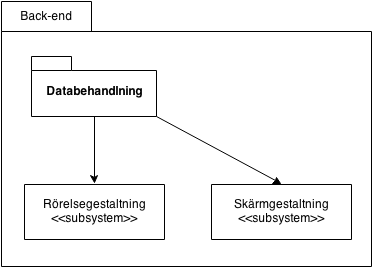
\includegraphics[scale=0.8]{backendorganizational.png}

\subsection{Designmetod}

\subsection{Komponent beskrivning}
SuperRecorder-SDK:t är utformat enligt <FIGURBETECKNING> \\

Klassen SuperRecorder är den centrala klassen i SDK:t och behåller primär kontroll under hela SDK:ts scope. SuperRecorder-klassen initialiserar samtliga andra moduler inom SDK:t och all intern kommunikation inom SDK:t förmedlas via denna klass. \\

GUI:t är den primära möjligheten för extern kommunikation till SDK:t. Genom GUI:t kan användaren ändra inställningar, starta/stoppa inspelning samt sända inspelning till servern. \\

ScreenRecorder ansvarar för inspelning av de aktiviteter som utförs av test-applikationen. Klassen sparar inspelningen i form av en fil som kan returneras vid förfrågan från SuperRecorder-klassen. SuperRecorder-klassen kan även begära start/stopp av inspelning. I övrigt har ScreenRecorder inga publika/package metoder. \\

TouchRecorder ansvarar för dokumentering av touch relevanta till de aktiviteter som utförs av test-applikationen. I övrigt är klassen extern sett att likställa med ScreenRecorder. \\

CameraRecorder ansvarar för inspelning av frontkameran under körning av test-applikationen. I övrigt är klassen extern sett att likställa med ScreenRecorder. \\

Sender sköter överföringen av media-filen till servern. \\

På servern konverteras media-filen till lämpligt format för lagring och uppspelning.

\section{Komponentbeskrivning}

\subsection{Kodintegrering} % (fold)
\label{sub:Kodintegrering}
\subsubsection{Typ}
Fristående program som förbehandlar testbeställarens applikation, och länkar samman denna med projektets moduler.

\subsubsection{Syfte}
Att snabbt och enkelt kunna integrera SuperRecorder SDK i ett nuvarande projekt för Android. Syftet relaterar direkt till URD 3.2.1.

\subsubsection{Funktionalitet}
Det finns två olika sätt som komponenten kan fungera på. Antingen är komponenten i form av ett mindre program, som testbeställaren laddar ner på sin egen dator. Programmet söker då igenom testbeställarens källkod, och modifierar den för att passa med projektets moduler. Kompilering sker sedan som vanligt, och applikationen skickas ut till testarnas mobiltelefoner. 

Ett annat alternativ är att länka samman testbeställarens applikation med SuperRecorder SDK efter kompilering. Detta sker genom så kallad dekompilering, för vilket verktyget \textit{apk-tool} är skapat. Om detta alternativ väljs skulle testbeställaren istället kunna skicka den kompilerade Android-applikationen till TBF:s servrar, där applikationen integreras med SuperRecorder och sedan skickas ut till testarna.

\subsubsection{Underordnade komponenter}
Komponenten har inga underordnade komponenter.

\subsubsection{Beroenden}
Verktyget \textit{apk-tool} och/eller lämpligt verktyg för automatiserad textbehandling.

\subsubsection{Gränssnitt}
Komponenten anropas en gång innan SuperRecorder kan exekvera, och har sedan inget gränssnitt mot det övriga systemet. 

\subsubsection{Resurser}
Komponenten behöver hela källkoden för den Android-applikation som ska testas, alternativt en kompilerad version av Android-applikationen i körbar form.

\subsubsection{Referenser}

\subsubsection{Process}
Processen är en sekventiell genomgång av källkod eller dekompilerad Android-bytekod. På ett antal ställen i koden läggs nya instruktioner till som anropar SuperRecorders programmoduler. Under exekvering av applikationen kommer senare SuperRecorder att ha tillgång till den data den behöver för att spela in testarens användarmönster.

\subsubsection{Data}
Komponenten behöver inte spara någon lokal data, utan använder sig bara av fördefinierade konstanter för att ändra på rätt delar av koden.


\subsection{Basaktivitet}
\subsubsection{Typ}
Java-klass
\subsubsection{Syfte}
Syftet med denna klass är att vara en mellanhand mellan applikationernas aktiviteter och klassen Activity. Detta behövs för att ta reda på vilken Activity som användaren befinner sig i under körning.
\subsubsection{Funktionalitet}
Klassen är menad att användas som superklass i varje aktivitet. När en aktivitet startas kallas basaktivitetens funktion onResume() som sparar undan en referens till aktiviteten. När en aktivitet avslutas kallas basaktvitetens funktion onDestroy() som i sin tur sätter referensen till null. Sistnämnda är mycket viktigt för att undvika massiva minnesläckor.
\subsubsection{Underordnade komponenter}
Alla aktiviteter till applikationen är underordnade komponenter. 
\subsubsection{Beroenden}
Inga beroenden
\subsubsection{Gränssnitt}
Denna komponent har inget direkt gränssnitt förutom den sparade referensen. Rörelse- och skärminspelning beror på den sparade referensen.
\subsubsection{Resurser}
Klassen implementerar Activity från Android SDK.
\subsubsection{Referenser}
Grundläggande kunskap om Android underlättar förståelsen av komponenten. Se http://developer.android.com
\subsubsection{Process}
Subkomponenterna, det vill säga testapplikationens aktiviteter, kallar på super.onResume() startar och super.onDestroy() i sina egna onResume() och onDestroy() funktioner. Dessa kallas när en aktivitet startar respektive avslutas. Vår basaktivitets kod kommer då att köras och kommer se ut ungefär som nedan.
\begin{verbatim}
protected void onResume() {
		set currentActivity to thisActivity;
}
protected void ondestroy() {
		set currentActivity to null;
}
\end{verbatim}
\subsubsection{Data}
 Komponenten har inga lokala data eller strukturer.


\subsection{Skärminspelning}
\subsubsection{Typ}
Java-klass
\subsubsection{Syfte}
Att ta skärmdumpar och skapa en JSON-fil med information om när dessa togs.
Se URD-krav 3.1.1
\subsubsection{Funktionalitet}
Klassen har publika funktioner för att starta och avsluta inspelning. Vid inspelning används basaktiviteten för att ta reda på vilken aktivitet som användaren befinner sig i. Skärmdumpar tas sedan från aktivitetens vyer så ofta som det är möjligt. Samtidigt sparas tidpunkterna vid varje skärmdump. När inspelningen avslutas sparas tidsinformationen ner i en JSON-fil och alla bilder i ett komprimerat format.
\subsubsection{Underordnade komponenter}
Inga underordnade komponenter
\subsubsection{Beroenden}
Skärminspelningskomponenten beror på basaktiviteten som ger oss möjlighet att veta vilken aktivitet som användaren befinner sig i.
\subsubsection{Gränssnitt}

\subsubsection{Resurser}
Förutom redan nämnt beroende krävs tillgång till Androids SDK.
\subsubsection{Referenser}

\subsubsection{Process}

\subsubsection{Data}


\subsection{Rörelser}
\subsubsection{Typ}
Java-klass

\subsubsection{Syfte}
På serversidan kommer olika delar kombineras för att generera en video som visar användarens test av applikationen. Rörelsehändelserna kommer representeras i form utav en text-fil med data. När videon sedan renderas kommer denna data användas för att rita ut rörelsehändelserna. \\
Komponenten ämnar uppfylla kravet ``Realtidsfingerrörelser'' (Se 3.2.4, URD-1).

\subsubsection{Funktionalitet}
När en inspelning startar börjar mobilen spara varje rörelsehändelse. Denna information sparas till en fil enligt JSON-standard. Exempel på den information som sparas är: \\
\begin{verbatim}
{timestamp=''1000'', interval=''17'', action=''up'', index=''0'', x=''310'', y=''670''}
\end{verbatim} 
\textbf{Timestamp} är tiden i millisekunder sedan inspelningen startade. Detta används för att kunna synka rörelsehändelserna med videon.

\textbf{Interval} är tiden sedan senaste rörelsehändelsen. Tiden anges i millisekunder.
 
 \textbf{Action} är vilken typ av rörelsehändelse det är. De tre vanligaste typerna är ``up'' när man släpper upp fingret, ``down'' när man placerar fingret på skärmen och ``move'' när man rör fingret över skärmen.
 
 \textbf{Index} är vilket finger på skärmen som står för rörelsehändelsen. $Index=0$ är det fingret som först nuddade skärmen, $index=1$ är andra fingret som nuddade skärmen, o.s.v. Detta gör det möjligt att rita ut rörelser som kommer från flera olika fingrar utan att blanda ihop dem.
 
 \textbf{X och Y} är den position fingret har i X- och Y-led.
 
\subsubsection{Underordnade komponenter}

\subsubsection{Beroenden}
Rörelsehändelserna kan skrivas i stort sett oberoende av andra komponenter. För använda informationen behövs dock en överföringsdel. Säkerheten i Android gör att inga utomstående applikationer eller användare har tillgång till filen som skrivits. Därför måste filen skickas till servern inifrån applikationen. Vid testning har skrivningen skett till externt lagringsmedium (SD-kort) istället.

Information som krävs är starttid för inspelningen samt själva rörelsehändelsen. Detta måste skickas från den activity som står för rörelsehändelsen, vilket kan fås från basaktiviteten.
\subsubsection{Gränssnitt}
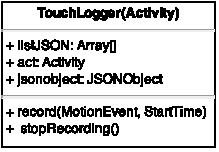
\includegraphics[scale=1.0]{TouchLogger.pdf}
\subsubsection{Resurser}
Kravet är att det finns en viss mängd minne för datafilen som genereras. Eftersom det rör sig om en textfil blir den aldrig speciellt stor.
\subsubsection{Referenser}
Denna komponent bygger på klassen MotionEvent.
\url{http://developer.android.com/reference/android/view/MotionEvent.html}
\subsubsection{Process}
Vid initiering av en activity skapas ett TouchLogger-objekt. 
\begin{verbatim}
TouchLogger tl;
\end{verbatim}
I onCreate()-metoden initieras TouchLogger-objektet med parametern \textbf{this}.
\begin{verbatim}
tl = new TouchLogger(this);
\end{verbatim}
Parametern \textbf{this} är activity:n som skickas med. Detta krävs för att sedan kunna skriva datan till en textfil. \\
För att sedan påbörja inspelning av rörelsehändelser kallas metoden record(MotionEvent event, float startTime). Metoden kallas från onTouchEvent(MotionEvent event) vilken är inbyggd i Android. Metoden kallas när den aktiva activity:n registrerar ett MotionEvent. 
\begin{verbatim}
if (recording) {
    tl.record(event, startTime);
}
\end{verbatim}
Event är den rörelsehändelse som ska spelas in och startTime är tidpunkten för inspelningens start. Denna tidpunkt behövs för att ge nyttig information (Såsom hur långt in i inspelningen denna rörelsehändelse ska dyka upp).

 För att avsluta inspelningen kallas metoden
 \begin{verbatim}
 tl.writeRecordToFile();
 \end{verbatim}
 vars syfte är att skriva datan till en textfil som sedan kan laddas upp till servern.
\subsubsection{Data}
Komponenten skapar ett JSON-objekt som sedan skriver detta objekt till en textfil vilken levereras till servern. Exempel hur filen kan se ut:
\begin{verbatim}
{``events'':
	``[{``timestamp'':''200'',interval=''17'',action=''down'',index=''0'',''x''=''310'',y=''670''},
	     {``timestamp'':''217'',interval=''17'',action=''move'',index=''0'',''x''=''320'',y=''680''},
	     {``timestamp'':''234'',interval=''17'',action=''up'',index=''0'',''x''=''330'',y=''700''}]''
}
\end{verbatim}

\subsection{Databehandling}
\label{sub:dataprocessing}
\subsubsection{Typ}
Servermodul som i huvudsak består av PHP-skript.

\subsubsection{Syfte}
Syftet med databehandlingsmodulen är att ta emot data från applikationstestaren i form av inspelade upplevelser av applikationen. Mottagen data innehåller, beroende på vad applikationstestaren spelat in; skärmdumpar, touch, ljud, inspelning från frontkameran samt diverse metadata om mobiltelefonen. Denna data sammanställs sedan där resultatet blir en film som sparas på servern samt data kring filmen och mobiltelefonen som sparas i en databas.

\subsubsection{Funktionalitet}
Data skickas från överföringsdelen via \texttt{HTTP}-protokollet genom metoden \texttt{POST} till servern där ett PHP-skript väntar. Mottagen data behandlas sedan av ett annat PHP-skript som använder submoduler för att sätta ihop skärmdumpar, touch, ljud och kamerainspelning till en video. Submodulerna returnerar en videofilm som sparas på servern. Till sist lagras information om videofilmen samt metadata från mobiltelefonen i en MySQL-databas.

\subsubsection{Underordnade komponenter}
Underordnade komponenter är \nameref{sub:touchmedia} och \nameref{sub:screenmedia}.

\subsubsection{Beroenden}
Denna modul kan komma att bero på PHP-ramverket Laravel. databehandlingen skapas i mån av tid som en insticksmodul till Laravel vilket skapar ett beroende till ramverkets kärnfiler som då måste finnas på servern.

\subsubsection{Gränssnitt}
Denna modul har inget användargränssnitt utan jobbar med \texttt{HTTP}-protokollet mot överföringsdelen.

\subsubsection{Resurser}
För att över huvud taget kunna använda denna modul krävs en servermiljö som kan exekvera PHP-skript och som har tillgång till en MySQL-databas. Dessutom krävs lagringsutrymme på servern för att kunna spara videofilmerna.

\subsubsection{Referenser}
Sektion 2.3.5 i URD-1 ger en motivering till varför sammansättning av media sker på serversidan istället för i mobiltelefonen. Sektion 2.6 i URD-1 handlar om servermiljön och under 2.6.2 ges en kort förklaring programmet FFmpeg som kommer att användas vid databehandlingen.

\subsubsection{Process}

\subsubsection{Data}


\subsection{Rörelsegestaltning}
\label{sub:touchmedia}
\subsubsection{Typ}

\subsubsection{Syfte}

\subsubsection{Funktionalitet}

\subsubsection{Underordnade komponenter}

\subsubsection{Beroenden}

\subsubsection{Gränssnitt}

\subsubsection{Resurser}

\subsubsection{Referenser}

\subsubsection{Process}

\subsubsection{Data}


\subsection{Skärmgestaltning}
\label{sub:screenmedia}
\subsubsection{Typ}

\subsubsection{Syfte}

\subsubsection{Funktionalitet}

\subsubsection{Underordnade komponenter}

\subsubsection{Beroenden}

\subsubsection{Gränssnitt}

\subsubsection{Resurser}

\subsubsection{Referenser}

\subsubsection{Process}

\subsubsection{Data}


\subsection{Kamerainspelning}
\subsubsection{Typ}
En modul som sköter videoinspelning från den främre kameran av testarens ansikte och sparar den till ett givet videoformat.

\subsubsection{Syfte}
Videoinspelning av ansiktet på den som testar applikationen är till för att ge en visuell bild av användaren samt att ytterligare ge information kring hur denna person upplever användargränsnittet på applikationen. Detta betyder att applikationsutvecklaren får mer information för att senare vidareutveckla sin produkt. Komponenter ämnar uppfylla kraven för Kamerainspelning (Se 3.1.3, URD-1).

\subsubsection{Funktionalitet}
Videoinspelning består utav 3 stycken klasser; Camera, MediaRecorder samt SurfaceView. Camera är det grundläggande API:t för att kontrollera kamerorna och används både för att ta bilder samt att spela in video. MediaRecorder klassen används för att spela in video från kameran. SurfaceView klassen visar en realtids förhandsvisning av vad kameran ser och visar det på skärmen. Den används alltså för att visa användaren vad kameran spelar in.

\subsubsection{Underordnade komponenter}
Ljudinspelning.

\subsubsection{Beroenden}
Den är inte beroende utav andra komponenter.

\subsubsection{Gränssnitt}


\subsubsection{Resurser}
För att kunna spela in med kameran så måste androidenheten först ha en framåtvänd kamera så att det går att spela in användarens ansikte under pågående test. Androidenheten bör också ha en nyare version av Android då alla funktioner kanske inte fungerar ifall enheten har en gammal version installerad.

\subsubsection{Referenser}
Kraven för Kamerainspelningen kan hittas under 3.1.3 i URD-1 men för att få en mer översiktlig insikt i hur kameran fungerar så kan man gå in på länken nedanför för att läsa om Kamera API:et för Androidutveckling.
http://developer.android.com/reference/android/hardware/Camera.html
http://developer.android.com/guide/topics/media/camera.html

\subsubsection{Process}
Det är en ganska avancerad process att starta en videoinspelning och alla delar måste starta i rätt ordning (Detta kan även läsas mer om i länken ovanför).
\begin{enumerate}
\item Öppna kameran för att få ett kamera objekt.
\item Förbered förhandvisning.
\item Starta förhandsvisningen.
\item Starta Videoinspelningen.
	\begin{enumerate}
		\item Lås upp kameran.
		\item Konfigurera MediaRecorder
		\begin{enumerate}
			\item Sätt kameran för videoinspelning, använd kamera objektet.
			\item Bestäm ljudkälla.
			\item Bestäm videokälla.
			\item Bestäm videoformat och kodning.
			\begin{enumerate}
				\item Bestäm videoformat.
				\item Bestäm ljudformat.
				\item Bestäm videokodnings typen.
			\end{enumerate}
			\item Bestäm utgående filformat.
			\item Bestäm förhandsvisnings utformningen för din applikation.
		\end{enumerate}
		\item Förbered MediaRecorder med givna inställningar.
		\item Starta MediaRecorder.
	\end{enumerate}
	\item Stoppa inspelning av video.
	\begin{enumerate}
		\item Stoppa MediaRecorder.
		\item Återställ Mediarecorder (valfri).
		\item Släpp lös MediaRecorder.
		\item Lås Kameran.
	\end{enumerate}
	\item Stoppa förhandsvisningen.
	\item Släpp lös kameran.
\end{enumerate}
Detta är hela förhandlingsloppet för att spela in en video med Camera, MediaRecorder och SurfaceView klasserna i Ansroid.

\subsubsection{Data}



\subsection{Ljudinspelning}
\subsubsection{Typ}
En modul som sköter ljudinspelning och sparar den som given ljudfil.

\subsubsection{Syfte}
Ändamålet för ljudinspelningsmodulen är att kunna spela in användarens röst under testning med SuperRecorder. Att höra användarens tankegångar under testning av användargränssnitt är högst önskvärt av apputvecklare. Komponenten ämnar uppfyllakravet Röstinspelning (Se 3.1.2, URD-1).

\subsubsection{Funktionalitet}
Ljudinspelningsmodulen har två publika metoder; void recordAudio och void stopRecording. RecordAudio kommer att kallas vid påbörjad inspelning med SuperRecorder och komma att köra tills dess att inspelningen avslutas av användaren genom StopRecording. När den senare kallas kommer ljudfilen skickas till given plats.

\subsubsection{Underordnade komponenter}
Denna komponent har inga underordnade komponenter.

\subsubsection{Beroenden}
Ljudinspelningen kommmer inte bero av någon annan komponent i projektet.

\subsubsection{Gränssnitt}
Gränssnittet till det övriga systemet fungerar genom att komponenten anropas genom recordAudio och stopRecording och producerar sedan en ljudfil som innehåller ljudet från mikrofonen.

\subsubsection{Resurser}
Ett krav är att det tillräckligt mycket minne för ljudfilen som genereras. Denna kommer dock inte vara stor.

\subsubsection{Referenser}
Under 3.1.2 i URD-1 finns en lista över funktionsmässiga krav för röstinspelningen i SuperRecorder.

\subsubsection{Process}
Från påbörjad inspelning sker inspelningen med hjälp av klassen MediaRecorder tills dess att användare avslutar inspelningen genom att MediaRecorder sköter ljudinspelningenstoppen och frigör resurser som använts vid inspelningen.

\subsubsection{Data}
Modulen består av objekt från klasserna MediaRecorder samt MediaPlayer. Den består också av en sökväg till platsen där ljudfilen ska sparas. Slutligen har modulen en boolsk variabel för att avgöra om objekten spelar in för tillfället.


\subsection{Komprimering}
\subsubsection{Typ}
En Java-klass som tar en eller flera filer och komprimerar samt arkiverar dem till en enda zip-fil. 

\subsubsection{Syfte}
När en betatestinspelning är slutförd genereras en mängd data som måste överföras till en server där den sammanställs för att sedan kunna presenteras för applikationsutvecklarna. Det är mer praktiskt att få all denna information i ett enda paket än att få alla filer skickade var för sig. Ju mindre filstorleken är desto mindre tid tar överföringen och mindre bandbredd används. Allt detta leder till att komprimering av data till en enda zip-fil utförs innan överföringen till servern sker. Detta relaterar till punkt 2.3.5 (sammansättning av media på serversidan) samt 2.3.6 (överföring) i URD:n. 

\subsubsection{Funktionalitet}
Klassen implementerar en publik metod \verb:zipFolder(): som tar två parametrar: en sökväg till mappen som ska komprimeras samt en sökväg till den komprimerade filen. Metoden går då rekursivt igenom alla filer och mappar, komprimerar dem och lägger till dem i en zip-fil. 

\subsubsection{Underordnade komponenter}
Inga underordnade komponenter

\subsubsection{Beroenden}
För att att klassen ska kunna komprimera filer krävs att filerna existerar samt att sökvägarna till filerna stämmer. 

\subsubsection{Gränssnitt}
Efter en slutförd inspelning av betatestning av en applikation genereras en mängd data som skrivs till filer. Dessa filer består av bland annat alla skärmdumpar som sedan ska sammanställas till en video, information om var användaren har tryckt på skärmen, videoinspelning av användarens ansikte, ljudinspelning av användaren med mera. Innan all data skickas till servern används denna klass för att komprimera filerna till en enda fil, som sedan skickas till servern. 

\subsubsection{Resurser}
Lagringsutrymme krävs för den genererade zip-filen. 

\subsubsection{Referenser}
Att lagra datan i flertalet filer i en enda, mindre fil kräver två steg: komprimering och arkivering. Komprimering leder till att en fil ockuperar mindre minnesutrymme (i detta fall på ett ickedestruktivt sätt, det vill säga det går att återskapa den ursprungliga datan utifrån den komprimerade datan) och arkivering innebär att flera filer lagras i en enda fil. \href{http://en.wikipedia.org/wiki/Gzip}{Gzip} är ett annat alternativ som ofta används vid komprimering, framförallt i Linuxmiljöer, vilket generar filer med filändelsen \verb:.gz:. Nackdelen med denna är att gzip inte stödjer arkivering, vilket oftast görs med programmet tar, och således är det vanligt att se komprimerade filer med filändelsen \verb:.tar.gz:. 

Zip stödjer både komprimering och arkivering, vilket är anledningen till att denna används. 

\subsubsection{Process}
Pseudokod: 
\begin{verbatim}
Class FileCompression {

	private constructor for non-instantiability

	public static  void zipFolder(String sourceFolderPath, String zipFilePath){
		Open outputStream
		addFolder(outputStream, sourceFolder, sourceFolder)
		Close outputStream
	}
	
	private static void addFolder(ZipOutputStream zos, String thisFilePath, String baseFolderPath){
		File f = new File(thisFilePath)
		
		if(f is a folder){
			if(f is a subfolder of baseFolder){
				add f as a folder entry in the zip-file, keeping the folder structure with root in baseFolder
				// Example: thisFilePath == ".../baseFolder/f1/f2/thisFolder"
				// In the zip-file, the folder entry /f1/f2/thisFolder/ will be created
			}
			for(every subfile in folder f){
				addFolder(zos, subfile, baseFolderPath)
			}
		} else {
			// f is a file, not a folder
			add f as a file entry in the zip-file, keeping the folder structure with root i baseFolder
			// Example: thisFilePath == ".../baseFolder/f1/f2/thisFile"
			// In the zip-file, the file entry /f1/f2/thisFile will be created
		}

	}
}
\end{verbatim}

\subsubsection{Data}
Klassen skapar en dataström per fil för indata samt en buffer för zip-filen som utdata. Sökvägarna till filerna fås genom argumenten i metoden \verb:public static  void zipFolder(String sourceFolderPath, String zipFilePath):. För varje fil i indatan skapas en ny dataström som läser in filen och sedan skrivs fildatan till en speciell buffer för zip-filen: \verb:ZipOutputStream out:. För varje infil skapas även en \verb:ZipEntry entry: som specificerar var i zip-filens mappstruktur som den inlästa filen ska läggas. Den slutgiltiga zip-filen producerar ett arkiv med mappstrukturen:
\begin{description}
  \item[Screenshots] \hfill \\
  	Skärmdumpar.
  \item[Touch] \hfill \\
  	JSON-filer med information om användarens fingerrörelser.
  \item[Video] \hfill \\
  	Videoinspelning av användaren.
  \item[Video] \hfill \\
  	Röstinspelning av användaren.
\end{description}

\subsection{Överföring}
\subsubsection{Typ}
Java-klass

\subsubsection{Syfte}
Att kunna överföra filer från applikationen på de mobila enheterna till en server. Detta relaterar till punkt 2.3.5 om mediasammansättning i URD:n, då sammansättningen sker på serversidan, samt punkt 2.3.6 om överföring. 

\subsubsection{Funktionalitet}
Klassen implementerar en metod som antingen tar en sträng som är sökvägen till filen som ska skickas, eller en lista med strängar till flera filer som ska skickas. Metoden öppnar sedan en anslutning till servern, skickar filerna med HTTP-protokollet med metoden POST och stänger sedan anslutningen till servern. 

\subsubsection{Underordnade komponenter}
Inga underordnade komponenter

\subsubsection{Beroenden}
För att denna klass ska kunna användas krävs att data från en inspelning av betatestning har genererats och sparats till filer. Att filerna är komprimerade och arkiverade enligt en förutbestämd fil- och mappstruktur är att föredra så att serversidan vet hur filerna ska extraheras och tolkas. Att en server finns som kan ta emot filer är såklart också ett krav. 

\subsubsection{Gränssnitt}
Efter en att en användare har slutfört sin betatesinspelning så genereras data om hur applikationen har använts. Datan sparas i filer som sedan komprimeras och arkiveras till en zip-fil. Denna fil måste sedan överföras till servern där de separata filerna som bl.a. innehåller skärmdumparna, användarens fingerrörelser, video- och ljudinspelning etc. sammanställs. 

\subsubsection{Resurser}
Ett lagringssystem på framförallt serversidan krävs för att kunna spara all information som genereras av betatestarna. 

\subsubsection{Referenser}
En anslutning mellan applikation och servern skapas genom TCP/IP-protokollen. Se \ref{tcp} och \ref{ip} för mer information. 

När en anslutning väl har etablerat används HTTP-protokollet, närmare bestämt en HTTP request med metoden POST för att skicka över en fil, enligt CRUD-principen (\ref{crud}). Mer om HTTP-protokollet finns i \ref{http}.

Den specifika implementation av dessa protokoll görs genom de inbyggda biblioteken i Java med klassen \verb:HttpUrlConnection:. 

\subsubsection{Process}
Pseudokod: 
\begin{verbatim}
Class FileTransfer
	public void send(String file){
		Open connection to server
		Read in file
		Send file
		Close connection to server
	}
	
	public void send(String[] files){
		Open connection to server
		for each file in files {
			Read in file
			Send file		
		}
		Close connection to server
	}
\end{verbatim}

\subsubsection{Data}
Klassen använder sig av två lokala dataströmmar: en som läser in zip-filen och en som skickar den inlästa datan till servern. Strömmen som läser in zip-filen fås genom: \verb:FileInputStream fileInputStream = new FileInputStream(new File(pathToOurFile) );: och strömmen som skickar över datan fås genom Java-objektet \verb:HttpURLConnection connection: som sköter anslutningen till servern: \verb:DataOutputStream outputStream = new DataOutputStream( connection.getOutputStream() );:. 

\subsection{GUI}
\subsubsection{Typ}
Samling av javaklasser och xml-dokument.
\subsubsection{Syfte}
URD-krav 4
URD-krav 6
GUI;t ansvarar för att möjliggöra visuell och fysisk interaktion mellan användaren och Super Recorder. 

\subsubsection{Funktionalitet}
GUI;t består av en mängd olika menyer som skickar information till GUI;t om att deras respektive knappar och liknande blivit tryckta. GUI;t är därav en komponent som endast tilldelar listeners för alla komponenter.

\subsubsection{Underordnade komponenter}
GUI Support, Huvudmeny, Settingsmeny, Inloggningsmeny, Videolista, Colorslider, Videomeny

\subsubsection{Beroenden}
För att GUI;t ska kunna användas behövs det en androidapplikation som implementerar funktionalitet för att kunna visa detta GUI. Androidapplikationen är i detta avseende den applikation som nyttjar detta projekts SDK för att kunna spela in användartestsessioner. GUI;t behöver även delar som ansvarar för att lagra inspelade testsessioner och diverse inställningar då dessa data inte lagras direkt i GUI;t.

\subsubsection{Gränssnitt}
GUI;t har ingen direkt kontakt med applikationen som har implementerat SDK;t. Applikationen begär att GUI;t ska visas, GUI;t kommer därefter att vara fortsatt aktivt fram till dess att GUI;t självt ger order om att tas bort. De externa komponenter GUI;t kommunicerar med är exklusivt den enda klass som är avsedd att lagra olika inställningsval samt skicka vidare olika begäran om att exempelvis starta en inspelning. Denna kommunikation är helt enkelriktad från GUI;t, inga anrop görs till GUI;t från externa komponenter. 

\subsubsection{Resurser}
Utöver det direkta beroende till Android är GUI;t i behov av en komponent som lagrar data GUI;t producerar samt skickar vidare eventuella begäran till rätt delar av programmet. GUI;t behöver även en androidapplikation för att kunna fungera.

\subsubsection{Referenser}
GUI;t är implementerat i Android och därav behövs kunskap om Android för att förstå komponenten.
http://developer.android.com/reference/packages.html

\subsubsection{Process}
GUI;t bistår med kontakt mellan alla subkomponenterna och ser till att dessa visas och placeras korrekt baserat på den önskade designen. Detta sker genom att lägga till listeners på alla subkomponenter, vilka behandlar alla interna händelser i subkomponter som är relevanta för andra komponenter i GUI;t  så att dessa händelser ger den effekt på GUI;t i sin helhet som de ska. I pseudukod kan det se ut som följande;
Void knapptryckt(knapp)
[…]
If knapp = knapp1
Then utför det som ska hända för knapp 1
If knapp = knapp2
Then utför det som ska hända för knapp 2
[…]

\subsubsection{Data}
GUI;t lagrar ingen intern data förutom det som följer genom användandet av Androids biblotek.

\subsection{GUI Support}
\subsubsection{Typ}
Java klass

\subsubsection{Syfte}
GUI Support är mellanhanden mellan GUI;t och alla andra komponenter i SDK;t som har direkt koppling med eventuella begäran från GUI;t. Detta innebär att de val kring inställningar som görs i GUI;t  samt alla inspelade testsessioner lagras i GUI Support.

\subsubsection{Funktionalitet}
GUI Support är en mellanhand som därav består av metoder för att hämta specifika data som exempelvis pekaren till listan av inspelade testsessioner eller för att ändra värden som specificerar inställningar för inspelningar. Den består även av metoder för att anropa rätt komponenter i SDK;t för att utföra önskade operationer vilket exempelvis kan vara att spela in en ny video.

\subsubsection{Underordnade komponenter}
Subkomponenter saknas.

\subsubsection{Beroenden}
För att GUI Support ska fungera måste det finnas en androidapplikation som har implementerat SDK;t.

\subsubsection{Gränssnitt}
GUI;t använder GUI Support för att hämta och förändra önskad data som sedan skickas vidare till andra komponenter som sköter inspelning.

\subsubsection{Resurser}
GUI Support behöver GUI för att fungera samt komponenter som kan sköta inspelning.

\subsubsection{Referenser}
Inga externa dokument är nödvändiga.

\subsubsection{Processer}
GUI Support består av getters och setter som anropas av GUI;t samt metoder som anropar metoder i andra externa komponenter.

\subsubsection{Data}
GUI Support lagrar en lista över alla inspelade testsessioner, en snapshot av vart i navigeringen GUI;t är, samt alla de värden som användaren kan ändra gällande inspelning.


\subsection{Inloggningsmeny}
\subsubsection{Typ}
Java klass och xml-dokument

\subsubsection{Syfte}
URD-krav 6
Visualiserar inloggningsmöjligheter i GUI;t. Den första menyn som visas vid visningen av GUI;t första gången. 

\subsubsection{Funktionalitet}
Inloggningsmenyn består av knappar, textfält för användarnamn samt lösenord, en knapp ska motsvara att en inloggningsrequest ska skickas och den andra att inloggningen skippas.

\subsubsection{Underordnade Komponenter}
Subkomponenter saknas.

\subsubsection{Beroenden}
GUI;t måste visas för att denna komponent ska vara relevant samt bör inloggningsservern vara i drift.

\subsubsection{Gränssnitt}
Vid tryckning på given knapp skickas information om att den specifika knappen tryckts till GUI;t.

\subsubsection{Resurser}
Inloggningsmenyn behöver GUI för att fungera.

\subsubsection{Referenser}
Inloggningsmenyn är implementerad i Android och därav behövs kunskap om Android för att förstå komponenten.
http://developer.android.com/reference/packages.html

\subsubsection{Processer}
För varje inputenhet tillskrivs följande listener:
If tryckt
then gui.inputenhetused(denna_inputenhet)

\subsubsection{Data}
Settingsmenyn lagrar ingen intern data förutom det som följer genom användandet av Androids biblotek.

\subsection{Huvudmeny}
\subsubsection{Typ}
Java klass och xml-dokument

\subsubsection{Syfte}
URD-krav 6
Visualiserar navigationsmöjligheter i GUI;t och tillhandahåller för användaren möjlighet att välja att spela in en testsession. 

\subsubsection{Funktionalitet}
Huvudmenyn består av knappar som skickar information om att de tryckts till GUI vilket sedan utför de händelser varje knapp  ska utlösa.

\subsubsection{Underordnade Komponenter}
Subkomponenter saknas.

\subsubsection{Beroenden}
GUI;t måste visas för att denna komponent ska vara relevant.

\subsubsection{Gränssnitt}
Vid knapptryckning skickas information om att den specifika knappen blivit tryckt till GUI.

\subsubsection{Resurser}
Huvudmenyn behöver GUI för att fungera.

\subsubsection{Referenser}
Huvudmenyn är implementerad i Android och därav behövs kunskap om Android för att förstå komponenten.
http://developer.android.com/reference/packages.html

\subsubsection{Prcocesser}
För varje knapp tillskrivs följande listener:
If tryckt
then gui.knapptryckt(dennaknapp)

\subsubsection{Data}
Huvudmenyn lagrar ingen intern data förutom det som följer genom användandet av Androids biblotek.

\subsection{Settingsmeny}
\subsubsection{Typ}
Java klass och xml-dokument

\subsubsection{Syfte}
URD-krav 4
URD-krav 6
Visualiserar navigationsmöjligheter i GUI;t och tillhandahåller för användaren möjlighet att välja vad som ska spelas in under en testsession. 

\subsubsection{Funktionalitet}
Settingsmenyn består av knappar, checkboxes och en färgväljare som skickar information om att de tryckts till GUI vilket sedan utför de händelser varje inputenhet ska utlösa.

\subsubsection{Underordnade Komponenter}
Colorslider.

\subsubsection{Beroenden}
GUI;t måste visas för att denna komponent ska vara relevant.

\subsubsection{Gränssnitt}
Vid tryckning på given inputenhet skickas information om att den specifika inputenheten blivit tryckt till GUI.

\subsubsection{Resurser}
Settingsmenyn behöver GUI för att fungera.

\subsubsection{Referenser}
Settingsmenyn är implementerad i Android och därav behövs kunskap om Android för att förstå komponenten.
http://developer.android.com/reference/packages.html

\subsubsection{Processer}
För varje inputenhet tillskrivs följande listener:
If tryckt
then gui.inputenhetused(denna_inputenhet)

\subsubsection{Data}
Settingsmenyn lagrar ingen intern data förutom det som följer genom användandet av Androids biblotek.

\subsection{Färgreglage}
\subsubsection{Typ}
Java klass och xml-dokument

\subsubsection{Syfte}
URD-krav 4
URD-krav 6
Möjliggöra för användaren att välja färg för visualiseringen av tryckningar för testsessioner.

\subsubsection{Funktionalitet}
Colorslidern består av en utritad färggradient. Vid tryckning på denna gradient kommer den färg som trycktes att skickas vidare till GUI;t.

\subsubsection{Underordnade Komponenter}
Subkomponenter saknas.

\subsubsection{Beroenden}
GUI;t måste visas för att denna komponent ska vara relevant.

\subsubsection{Gränssnitt}
Genom att lägga till en listener till Colorslidern kommer denna komponent att skicka information om vilken färg som tryckts på till alla listeners. 

\subsubsection{Resurser}
Det behövs något objekt som lagt till en listener till Colorslidern.

\subsubsection{Referenser}
Inga externa dokument är nödvändiga.

\subsubsection{Processer}
Vid skapandet räknas en färggradient ut baserat på längden på slidern och lagras. Vid tryckning på colorsiden hämtas sedan färgen ut för det tryckta x-värdet och skickas till alla listeners.

\subsubsection{Data}
En lokal färggradient lagras.

\subsection{Videolista}
\subsubsection{Typ}
Java klass och xml-dokument

\subsubsection{Syfte}
URD-krav 6
Visualiserar vilka inspelningar som finns lagrade i SuperRecorder.

\subsubsection{Funktionalitet}
Videolistan består av en scrollbar lista som visualiserar mängden av alla inspelningar som finns lagrade i Super Recorder. Det finns dessutom en knapp som ska motsvara att backa till huvudmenyn. Vid tryckning på ett element i listan skall detta begära en meny där detta objekt kan behandlas.

\subsubsection{Underordnade Komponenter}
Subkomponenter saknas.

\subsubsection{Beroenden}
GUI:t måste visas för att denna komponent ska vara relevant. Dessutom måste en pekare till den plats i minnet där videorna för testsessionerna finnas tillgänglig.

\subsubsection{Gränssnitt}
Vid tryckning på given inputenhet skickas information om att den specifika inputenheten tryckts till GUI:t. Ifall ett element i listan trycks så skickas informationen att det specifika elementet har trycks.

\subsubsection{Resurser}
Videolistan behöver GUI för att fungera.

\subsubsection{Referenser}
Videolistan är implementerad i Android och därav behövs kunskap om Android för att förstå komponenten.
\url{http://developer.android.com/reference/packages.html}

\subsubsection{Processer}
För varje inputenhet tillskrivs följande listener:
\begin{verbatim}
If tryckt
then gui.inputenhetused(denna_inputenhet)
\end{verbatim}

\subsubsection{Data}
Videolistan lagrar ett Adapter-objekt som kan upptäcka om förändringar har skett i listan som lagrar inspelade testsessioner. Förutom det lagras ingen intern data förutom det som följer genom användandet av Androids biblotek.


\subsection{Videomeny}
\subsubsection{Typ}
Java klass och xml-dokument

\subsubsection{Syfte}
URD-krav 6
Tillhandahåller för användaren möjlighet att göra val kring en redan inspelad testsession.

\subsubsection{Funktionalitet}
Menyn består av en knapp som betyder att videon ska spelas upp, en för att ta bort videon samt en för att ladda upp. Uppladdningsknappen kan endast tryckas på ifall användaren är inloggad och att videon inte redan är uppladdad. Slutligen finns det en knapp för navigation tillbaka till videolistan.

\subsubsection{Underordnade Komponeter}
Subkomponenter saknas.

\subsubsection{Beroenden}
Det måste existera en inspelad testsession samt att denna inspelning måste vara utpekad som den inspelning som ska visas i denna meny. Dessutom måste GUI:t visas för att denna komponent ska vara relevant.

\subsubsection{Gränssnitt}
Vid knapptryckning skickas information om att den specifika knappen blivit tryckt till GUI.

\subsubsection{Resurser}
Videomenyn behöver GUI för att fungera.

\subsubsection{Referenser}
Videomeyn är implementerad i Android och därav behövs kunskap om Android för att förstå komponenten.
\url{http://developer.android.com/reference/packages.html}

\subsubsection{Processer}
För varje knapp tillskrivs följande listener:
\begin{verbatim}
If tryckt
then gui.knapptryckt(denna_knapp)
\end{verbatim}

\subsubsection{Data}
Videomenyn lagrar ingen intern data förutom det som följer genom användandet av Androids biblotek.

\section{Genomförbarhetsstudie}
\label{sec:estimates}

\subsection{Minimum} % (fold)
\label{sub:Minimum}

Ett antal av de definierade komponenterna relaterar direkt till projektets ``minimum-behov''. Detta innebär att komponenterna är essentiella för att projektet ska uppnå utlovad funktionalitet. Komponenterna som faller inom denna kategori är \textit{skärminspelning}, \textit{rörelser} \textit{röstinspelning}, \textit{kamerainspelning}. Alla dessa har redan färdiga prototyper som fungerar väl på egen hand, kvarvarande uppgift är därför att sätta ihop modulerna till ett system. Androids interna systembeteende har visat sig försvåra vissa typer av externa anrop, exempelvis kan \textit{skärminspelning} i nuvarande form kollidera med Androids egna grafikkod och medföra krascher och/eller försämrad prestanda. Problem likt dessa har dock inte varit lika framträdande i övriga ``minimum-moduler''. Gruppen har därför goda skäl att tro att dessa moduler har möjlighet att fungera tillräckligt bra tillsammans för att önskvärd funktionalitet ska uppnås.

\subsection{Standard} % (fold)
\label{sub:Standard}

Komponenter som sträcker sig utanför de allra mest grundläggande kraven, men ändå är viktiga för en godtagbar användarupplevelse, faller inom ``standard-behov''. Komponenterna inom denna kategori är övriga definierade komponenter, utom de som redan blivit indelade i ``minimum"-kategorin''. Även många komponenter i ``standard''-kategorin har färdiga prototyper som har visat sig fungera väl i avskiljda testmiljöer. Det är i denna kategori dock inte lika självklart att komponenter fungerar bra nog tillsammans för att uppnå tillräcklig prestanda. Speciellt projektets komponenter på server-sidan, \textit{databehandling} med \textit{rörelsegestaltning} och \textit{skärmgestaltning}, utför en tyngre sorts beräkningar som troligen behöver optimeras från den nuvarande prototyp-formen. Uppskattningsvis tar sammanställningen av en video av längd $n$ sekunder mellan $0,{}75n$ och $n$ sekunder på modern hårdvara. Detta kan vara ohållbart i en storskalig miljö med flera simultana användare.

Värt att nämna är dock att dessa uppskattningar baserar sig på körning av enklare prototypmoduler, som har utvecklats av ett fåtal gruppmedlemmar och med låg arbetsprioritet. Då den ursprungliga projektplanen i PPD-1 har följts med avseende på mjukvaru-utveckling har flera gruppmedlemmar frigjorts för att kunna arbeta tillsammans på de komplexare ``standard-modulerna''. Detta bådar gott för att den dedikerade utvecklingstiden till dessa komponenter ska räcka för att optimera körningen tillräckligt.

\subsection{Övrigt} % (fold)
\label{sub:Ovrigt}

Komponenten \textit{kodintegration} tillför inte projektet någon ny funktionalitet, utan syftar endast till att underlätta integrationen mellan SuperRecorder SDK och testbeställarens egen Android-applikation. Komponenten har därför tillägnats en låg prioritet, även om den direkt är kopplad till ett ursprungligt krav från projektbeställarna. Gruppens befintliga research i frågan tyder på att en enklare version som fungerar för majoriteten av fallen är klart genomförbar inom tidsspannet för utvecklingsfasen. Det är däremot oklart ifall tid finns för att testa och utvidga komponenten till en mera robust lösning. Möjligen blir alternativet att erbjuda tjänsten till slutkund, för att senare hänvisa dessa till manuell integrering om komponenten inte fungerar för just deras fall.

% subsection Integration (end)

\subsection{Tidsplan}
\begin{figure}[H]
\centering
\begin{tabular}{ | l | l | l |}
  \hline
  \textbf{Systemmodul} & \textbf{Deadline} & \textbf{Uppskattad tidsåtgång} \\ \hline
  GUI & 6/4 & 30h \\ \hline
  GUI Support & 6/4 & 10h \\ \hline
  Inloggningsmeny & 6/4 & 10h \\ \hline
  Huvudmeny & 6/4 & 10h \\ \hline
  Settingsmeny & 6/4 & 5h \\ \hline
  Färgreglage & 6/4 & 5h \\ \hline
  Rörelser & 6/4 & 10h \\ \hline
  Rörelsegestaltning & 6/4 & 30h \\ \hline
  Kamerainspelning & 6/4 & 20h \\ \hline
  Ljudinspelning & 6/4 & 5h \\ \hline
  Videomeny & 4/5 & 10h \\ \hline
  Videolista & 4/5 & 40h \\ \hline
  Basaktivitet & 4/5 & 50h \\ \hline
  Databehandling & 4/5 & 50h \\ \hline
  Skärminspelning & 4/5 & 300h  \\ \hline
  Skärmgestaltning & 4/5 & 300h \\ \hline
  Komprimering & 4/5 & 200h \\ \hline
  Överföring & 4/5 & 200h \\ \hline
\end{tabular}
\caption*{\textit{Komponent-deadlines}}
\end{figure}

\section{User Requirements vs Components Traceability Matrix}
\label{sec:user_req}

\begin{figure}[H]
\centering
\begin{tabular}{ | l | l | l | l | l | l | l | l |}
  \hline
    & UR-3.1.1 & UR-3.1.2 & UR-3.1.3 & UR-3.1.4 & UR-3.1.5 & UR-3.2.4 & UR-3.2.6\\ \hline
   AR-5.1 & X &  &  &  & X &  & \\ \hline
   AR-5.2 & X &  &  &  &  &  &  \\ \hline
   AR-5.3 &  &  &  &  & X & X &  \\ \hline
   AR-5.4 &  &  &  &  &  &  &  \\ \hline
   AR-5.5 &  &  &  &  &  & X &  \\ \hline
   AR-5.6 &  &  &  &  &  &  &  \\ \hline
   AR-5.7 &  &  & X &  &  &  &  \\ \hline
   AR-5.8 &  & X &  &  &  &  &  \\ \hline
   AR-5.9 &  &  &  &  &  &  &  \\ \hline
   AR-5.10 &  &  &  &  &  &  &  \\ \hline
   AR-5.11 &  &  &  &  &  &  & X \\ \hline
   AR-5.12 & &  &  & X & X &  & X \\ \hline
   AR-5.13 &  &  &  &  &  &  & X \\ \hline
   AR-5.14 &  &  &  &  &  &  & X \\ \hline
   AR-5.15 &  &  &  & X &  &  & X \\ \hline
   AR-5.16 &  &  &  &   &  &  & X \\ \hline
   AR-5.17 &  &  &  &  &  &  & X \\ \hline
   AR-5.18 &  &  &  &  &  &  & X \\ \hline
\end{tabular}
\end{figure}

\printbibliography[heading=bibintoc] % bibliography in table of contents

\renewcommand{\appendixtocname}{Appendix}
\renewcommand{\appendixpagename}{Appendix}
\begin{appendices}

\addcontentsline{toc}{section}{A Mötesprotokoll}
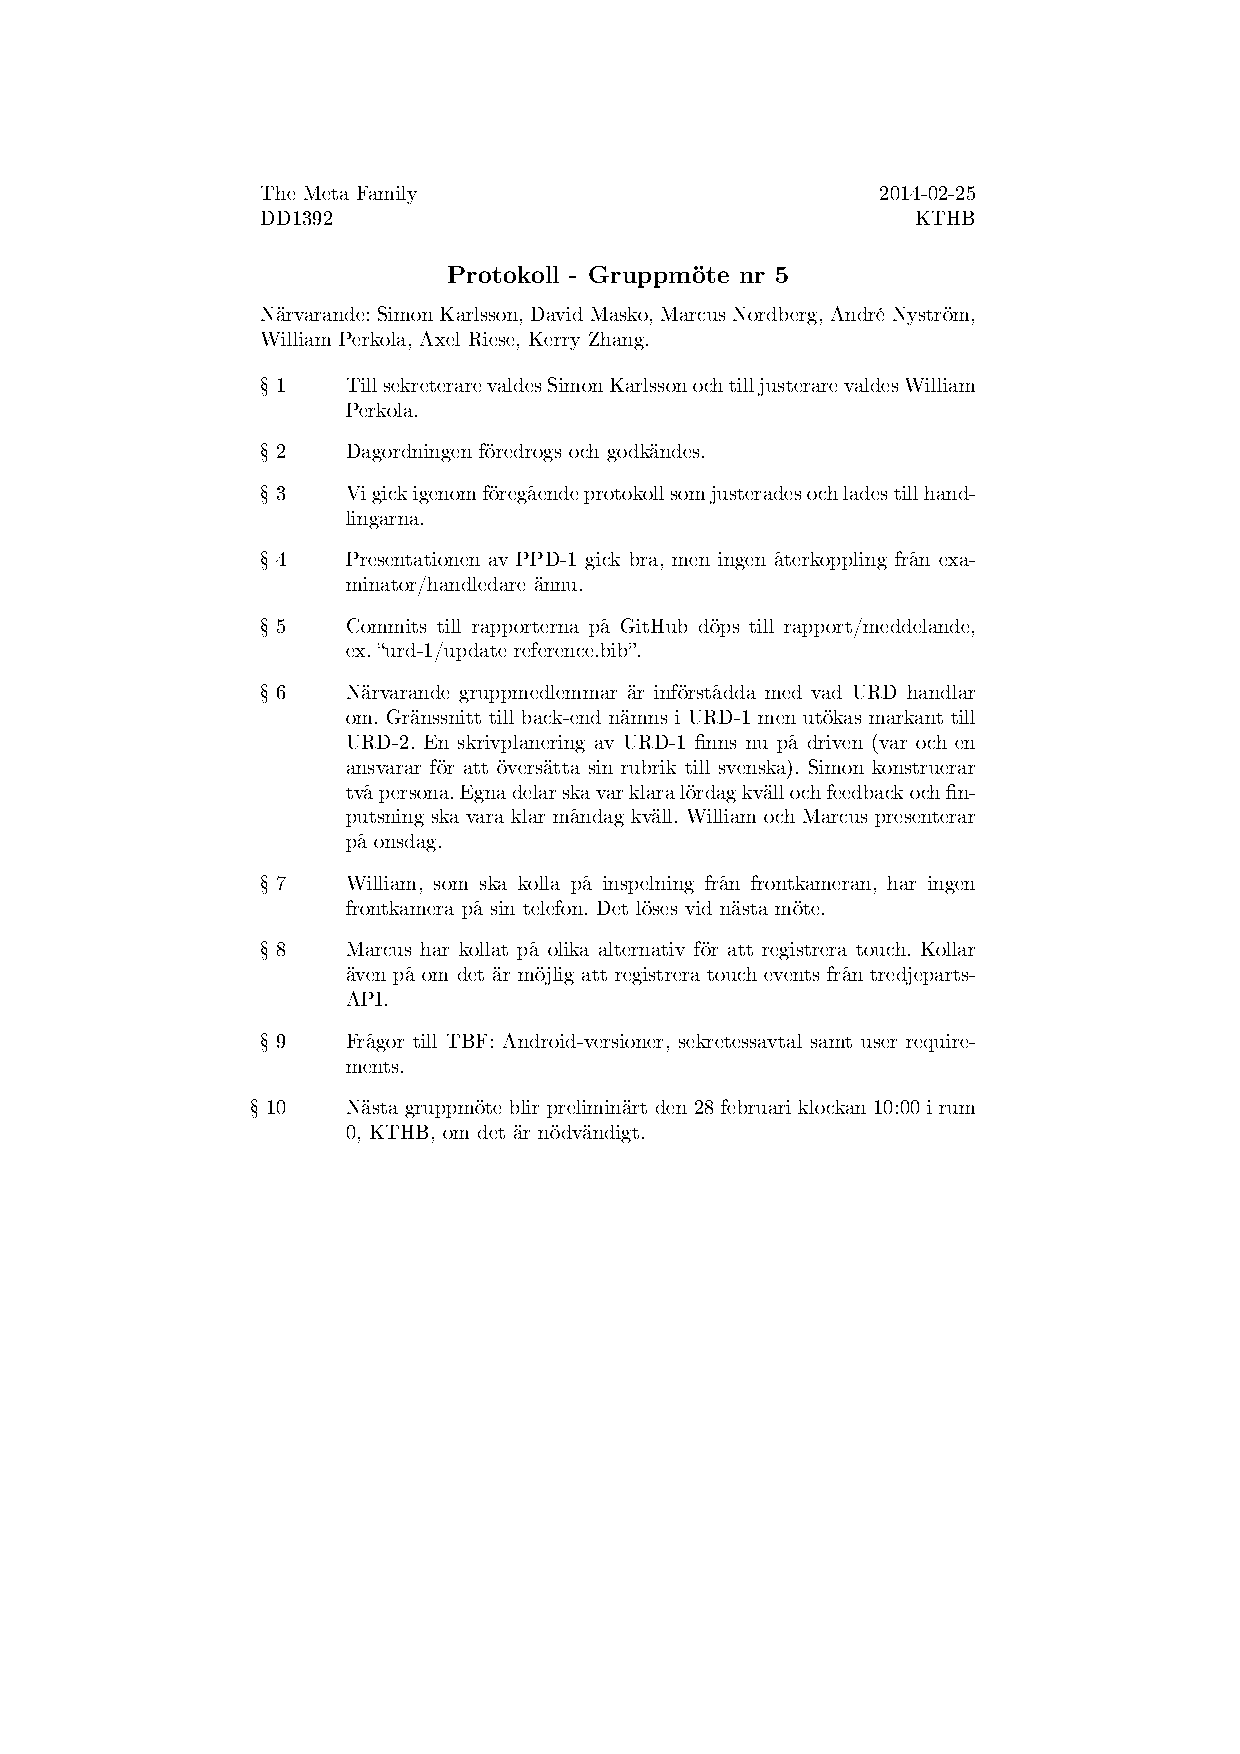
\includepdf{protokoll_2014-02-25}

\end{appendices}

\end{flushleft}
\end{document}
